
% This LaTeX was auto-generated from an M-file by MATLAB.
% To make changes, update the M-file and republish this document.

\documentclass{article}
\usepackage{graphicx}
\usepackage{color}

\sloppy
\definecolor{lightgray}{gray}{0.5}
\setlength{\parindent}{0pt}

\begin{document}

    
    
\subsection*{Contents}

\begin{itemize}
\setlength{\itemsep}{-1ex}
   \item * Set up the Laplacian Matrix x-direction
   \item * Combine lap with identity matrix
   \item Initialize Source function
   \item * Initialize loop and plot variables
   \item * Loop over desired number of steps (wave circles system once)
   \item Plot
\end{itemize}
\begin{verbatim}
% TwoDHeatEquation - Program to solve the diffusion equation
% using the Backward Euler method
clear; help TwoDHeatEquation; % Clear memory and print header

%* Initialize parameters (time step, grid spacing, etc.)
tau = 0.05; % Enter time step
N = 100; % Number of grid points
L = 1; % The system extends from (x,y)=(0,0) to (x,y)=(L,L)
h = L/N;
i = 0:(N-1);
j = 0:(N-1);
x = h/2 + i*h;
y = h/2 + j*h;
w = 0.2;
xs = 0.5;
ys = 0.5;
\end{verbatim}

        \color{lightgray} \begin{verbatim}  TwoDHeatEquation - Program to solve the diffusion equation
  using the Backward Euler method

\end{verbatim} \color{black}
    

\subsection*{* Set up the Laplacian Matrix x-direction}

\begin{verbatim}
lap = zeros(N);  % Set all elements to zero
coeff = 1/h^2;
for i=2:(N-1)
    for j=2:(N-1)
        lap(i,i-1,j) = coeff;
        lap(i,i,j) = -4*coeff;  % Set interior rows
        lap(i,i+1,j) = coeff;
        lap(i,i,j-1) = coeff;
        lap(i,i,j+1) = coeff;
    end
end
lap(1,1,1)=-coeff;
lap(1,2,2)=coeff;
lap(N,N,N)=-coeff;
lap(N,N-1,N-1)=coeff;
iMatrix=zeros(N,N,N);
iMatrix(1:1+N+N^2:end)=1;
\end{verbatim}


\subsection*{* Combine lap with identity matrix}

\begin{verbatim}
dM = iMatrix - tau*lap;
\end{verbatim}


\subsection*{Initialize Source function}

\begin{verbatim}
S = zeros(N); % Set all elements to zero
xExponent = (x'-xs).^2;
yExponent = (y-ys).^2;
S = exp(-xExponent/w^2);
Q0 = S;
S3D = exp(-xExponent/w^2)*exp(-yExponent/w^2);
mesh(S3D);
\end{verbatim}

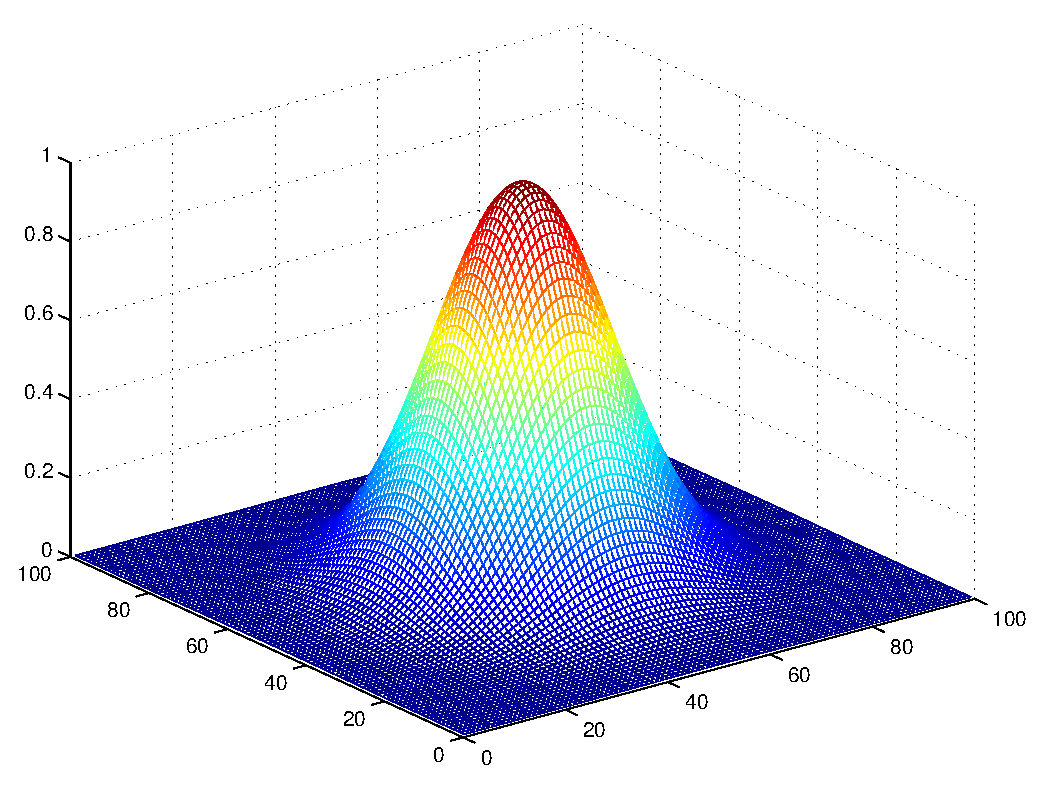
\includegraphics [width=4in]{TwoDHeatEquation_01.eps}


\subsection*{* Initialize loop and plot variables}

\begin{verbatim}
max_iter = .5/tau;
time = linspace(0,max_iter*tau,max_iter);
Qplot(:,1) = S; % initial value set to source
\end{verbatim}


\subsection*{* Loop over desired number of steps (wave circles system once)}

\begin{verbatim}
for iter=2:round(.25/tau)
    %* Compute new temperature
    Q0 = dM\(Q0)+S;
    Qplot(:,iter) = Q0(:);
end
for iter=round(.25/tau):max_iter
    %* Compute new temperature
    Q0 = dM\(Q0);
    Qplot(:,iter) = Q0(:);
end
\end{verbatim}

        \color{lightgray} \begin{verbatim}Error using \
Inputs must be 2-D, or at least one input must be scalar.
To compute elementwise LDIVIDE, use LDIVIDE (.\) instead.

Error in TwoDHeatEquation (line 54)
    Q0 = dM\(Q0)+S;
\end{verbatim} \color{black}
    

\subsection*{Plot}

\begin{verbatim}
figure(2);clf;
mesh(time(length(time)/2:end),x,Qplot(:,length(time)/2:end));
xlabel('t'); ylabel('x');
\end{verbatim}



\end{document}
    
